\documentclass[12pt]{article}
% include the pckage of the color%
\usepackage[usenames, dvipsnames]{color}
\usepackage[english]{babel}
\usepackage[utf8x]{inputenc}
\usepackage{amsmath}
\usepackage{graphicx}

%define your own color %
\definecolor{mygray}{gray}{0.9}

\begin{document}
	\listoffigures
	
	\title{Chapter 4 : Implementation}
	\maketitle
	\section{Introduction}
	
	In this chpater we will focus on the technologies. 
	\section{Java Platform, Enterprise Edition (Java EE)}
	\begin{figure}[h]
		\centering
		
\includegraphics[width=0.4\textwidth]{JAVAEE_logo.png}
		\caption{Java Enterprise Edition logo}
		
	\end{figure}
	\vspace{66mm}
	\section{Angular JS}
	\begin{figure}[h]
		\centering
		
\includegraphics[width=0.3\textwidth]{AngularJS_logo.png}
		\caption{AngularJS logo}
	\end{figure}
	\subsection{Introduction}
	AngularJS is a structural framework for dynamic web apps. It lets you use HTML as your template language and lets you extend HTML's syntax to express your application's components clearly and succinctly. AngularJS's data binding and dependency injection eliminate much of the code you would otherwise have to write.  And it all happens within the browser, making it an ideal partner with any server technology.
	\\
	\\
	AngularJS is what HTML would have been, had it been designed for applications. HTML is a great declarative language for static documents. It does not contain much in the way of creating applications, and as a result building web applications is an exercise \textit{in what do I have to do to trick the browser into doing what I want?}
	\\
	\\
	The impedance mismatch between dynamic applications and static documents is often solved with:
	\begin{itemize}
		
		\item \textbf{a library} - a collection of functions which are useful when writing web apps. Your code is in charge and it calls into the library when it sees fit. E.g., \colorbox{mygray}{jQuery}.
		\item \textbf{frameworks} - a particular implementation of a web application, where your code fills in the details. The framework is in charge and it calls into your code when it needs something app specific. E.g., \colorbox{mygray}{durandal}, \colorbox{mygray}{ember}, etc.
	\end{itemize}
	AngularJS takes another approach. It attempts to minimize the impedance mismatch between document centric HTML and what an application needs by creating new HTML constructs. AngularJS teaches the browser new syntax through a construct we call directives. Examples include:
	\begin{itemize}
		\item Data binding, as in \colorbox{mygray}{\{\{\}\}}
		\item DOM control structures for repeating, showing and hiding DOM fragments.
		\item Support for forms and form validation.
		\item Attaching new behavior to DOM elements, such as DOM event handling.
		\item Grouping of HTML into reusable components.
		
	\end{itemize}	
	
	
	\subsection{Features}
	this section include the features
	\subsection{Motivation}
	this section include the features
	
	\section{Bootstrap}
	\begin{figure}[h]
		\centering
		
\includegraphics[width=0.20\textwidth]{Boostrap_logo.png}
		\caption{Bootstrap logo}
	\end{figure}
	\subsection{Introduction}
	\textbf{Bootstrap} is a free and open-source front-end web framework for designing websites and web applications. It contains HTML- and CSS-based design templates for typography, forms, buttons, navigation and other interface components, as well as optional JavaScript plugins. Unlike many web frameworks, it concerns itself with front-end development only.
	\\
	\\
	Bootstrap was developed by Mark Otto and Jacob Thornton at Twitter, and released as an open source product in August 2011 on GitHub.\\
	\textbf{In June 2014 Bootstrap was the No.1 project on GitHub!}
	\subsection{Features}
	\textbf{Bootstrap 3} supports the latest versions of the \textbf{Google Chrome}, \textbf{Firefox}, \textbf{Internet Explorer}, \textbf{Opera}, and \textbf{Safari} (except on Windows). It additionally supports back to IE8 and the latest Firefox Extended Support Release (ESR).
	\\
	Since \textbf{2.0}, \textbf{Bootstrap} supports \textbf{responsive web design}. This means the layout of web pages adjusts dynamically, taking into account the characteristics of the device used (desktop, tablet, mobile phone).
	\\
	Starting with \textbf{version 3.0}, Bootstrap adopted a mobile-first design philosophy, emphasizing responsive design by default.
	\\
	The \textbf{version 4.0} alpha release added \textbf{Sass} and \textbf{flexbox} support
	\subsection{Motivation}
	All the researchs shows that Bootstrap The most popular HTML, CSS, and JavaScript framework for developing responsive, mobile first projects on the web.
	\\
	According to github, Bootstrap is the second starred repository, with \textbf{115k stars}.
	\begin{figure}[h]
		\centering
		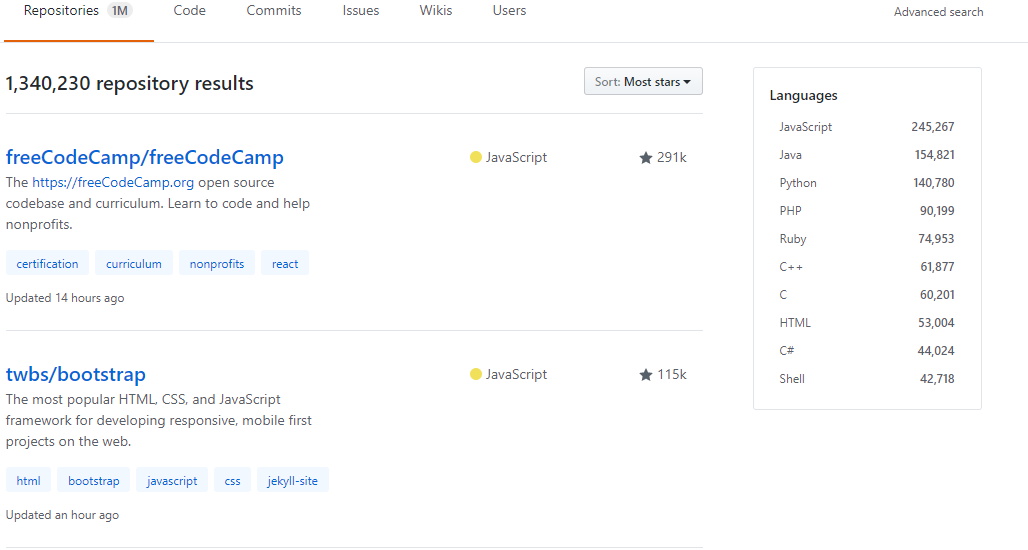
\includegraphics[width=1\textwidth]{Boostrap_statics_github.png}
		\caption{Bootstrap second starred on github}
	\end{figure}
	
	\vspace{66mm}
	
	According to a researchs, did it by myself in the net, all the high-tech blogs encourage developers to use bootstrap.
	\\
	\\
	I used a tool offred by google named \textbf{google trends} to make a compraison between a subjects in term of most researched.
	\\
	After this compraison in google trends, Bootstrap also is the most googled css framework on the web , compared to the others css frameworks Eg. \textbf{Material UI} which was considered as the most popular css framework after Bootstrap.
	
	\begin{figure}[h]
		\centering
		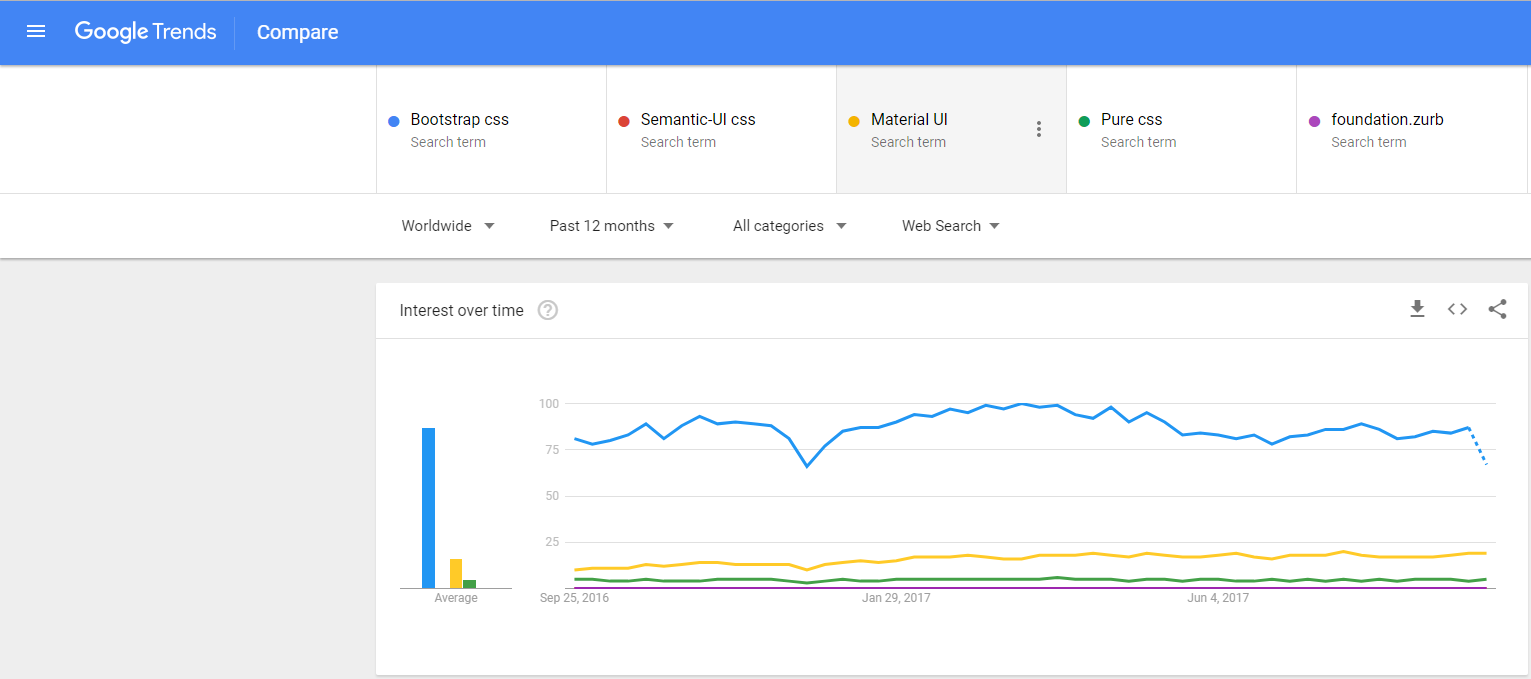
\includegraphics[width=1\textwidth]{Boostrap_statics_google_trends.png}
		\caption{Bootstrap on google trends}
	\end{figure}
	\vspace{66mm}
	\section{Spring mvc framework}
	\begin{figure}[h]
		\centering
		
\includegraphics[width=0.4\textwidth]{Spring_logo.png}
		\caption{Spring logo}
	\end{figure}
	\subsection{Introduction}
	The Spring Web model-view-controller (MVC) framework is designed around a \colorbox{mygray}{DispatcherServlet} that dispatches requests to handlers, with configurable handler mappings, view resolution, locale, time zone and theme resolution as well as support for uploading files. The default handler is based on the \colorbox{mygray}{@Controller} and \colorbox{mygray}{@RequestMapping} annotations, offering a wide range of flexible handling methods. With the introduction of Spring 3.0, the \colorbox{mygray}{@Controller} mechanism also allows you to create RESTful Web sites and applications, through the \colorbox{mygray}{@PathVariable} annotation and other features.
	\\
	\\
	Spring’s web MVC framework is, like many other web MVC frameworks, request-driven, designed around a central Servlet that dispatches requests to controllers and offers other functionality that facilitates the development of web applications. Spring’s \colorbox{mygray}{DispatcherServlet} however, does more than just that. It is completely integrated with the Spring IoC container and as such allows you to use every other feature that Spring has.
	\\
	\\
	The request processing workflow of the Spring Web MVC \colorbox{mygray}{DispatcherServlet} is illustrated in the following diagram. The pattern-savvy reader will recognize that the \colorbox{mygray}{DispatcherServlet} is an expression of the ``Front Controlle'' design pattern (this is a pattern that Spring Web MVC shares with many other leading web frameworks).
	\begin{figure}[h]
		\centering
		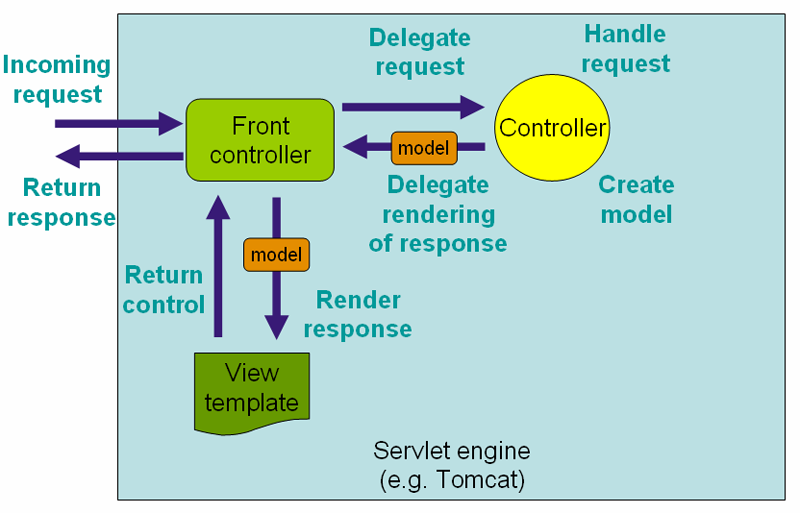
\includegraphics[width=1.0\textwidth]{workflow_spring_mvc.png}
		\caption{The request processing workflow in Spring Web MVC}
	\end{figure}
	
	\section{Apache Maven}
	\begin{figure}[h]
		\centering
		
\includegraphics[width=0.5\textwidth]{Maven_logo.png}
		\caption{Apache Maven logo}
	\end{figure}
	\section{HTML5}
	\begin{figure}[h]
		\centering
		
\includegraphics[width=0.3\textwidth]{HTML5_logo.png}
		\caption{HTML5 logo}
	\end{figure}
	\section{CSS3}
	\begin{figure}[h]
		\centering
		
\includegraphics[width=0.3\textwidth]{CSS3_logo.png}
		\caption{CSS3 logo}
	\end{figure}
\end{document}